% Para facilitar a manutenção é sempre melhore criar um arquivo por capitulo, para exemplo isso não é necessário 

%---------------------------------------------------------------------------------------

%---------------------------------------------------------------------------------------


\chapter{Materiais e Métodos}
Segundo \citeonline{Junior:2010}, engenharia de \textsl{software} é ``um conjunto integrado de métodos e ferramentas utilizadas para especificar, projetar, implementar e manter um sistema'', e que, para tanto, reúne em si metodologias, métodos e ferramentas para que o projeto seja bem definido em todas as suas etapas, variando desde sua problemática inicial e indo até sua entrega enquanto um produto de \textsl{software}. É a partir disto, que \citeonline{Junior:2010} distingue um método de uma ferramenta:

\begin{citacao}

Um método é uma prescrição explícita de como chegar a uma atividade requerida por um modelo de ciclo de vida, visando otimizar a execução das atividades que foram especificadas. Já as ferramentas proporcionam apoio automatizado ou semi-automatizado aos métodos\cite{Junior:2010}.

\end{citacao}

Ademais, \citeonline{Junior:2010} ainda separa os métodos de desenvolvimento de sistema em três categoriais que permitem visualizar e solucionar o problema de diferentes maneiras para sua modelagem. Para a composição do presente projeto, no entanto, será utilizado como método principal a metodologia escolhida para a gestão do projeto e as ferramentas poderão ou não ser relacionadas a mesma, como há de ser especificado nas próximas seções.
%---------------------------------------------------------------
\section{Tecnologias e ferramentas de desenvolvimento}

Pensando no objetivo e alcance do projeto, decidimos por realizar uma aplicação Web inicialmente, a qual pode ser acessada de diferentes dispositivos de forma fácil, apenas sendo necessário o acesso à \textit{internet}. Outros fatores considerados são a experiência da equipe com o mesmo e a disponibilidade de conteúdo sobre desenvolvimento Web.

De modo a desenvolver essa aplicação, será usado \acs{html}, \acs{css} e JavaScript como base para o \textsl{\gls{front-end}}, já os \glspl{framework2} que servirão de auxílio serão o \gls{react-bootstrap} e o \gls{ant}. 

Para o \textsl{\gls{back-end}} foi considerada a linguagem Java, orientada a objetos; sua escolha foi feita pelo fato da equipe já possuir experiência com a linguagem, além de alguns já trabalharem com a mesma, ela também possui uma boa maturidade, contendo muitas informações disponíveis para ajudar no desenvolvimento. Em conjunto, será utilizado \textit{Spring Boot}: \gls{framework2} Java de código aberto, e será juntamente usado o \textit{Maven}: \gls{framework2} de automação e gerenciamento de dependências no projeto.  Já como padrão de desenvolvimento utilizado no  \textsl{\gls{back-end}}, será aplicado o padrão \acs{mvc}, que separa o projeto em três principais camadas, \textit{model}, \textit{view} e \textit{controller}.

No entanto, como arquitetura de sistema, foi escolhido utilizar a arquitetura \gls{REST API} na qual é possível separar o código \textsl{\gls{back-end}} do \textsl{\gls{front-end}} de maneira que as duas aplicações possam determinar a troca informações entre elas com requisições via protocolo \acs{http}. Está solução também é útil para escalonar a plataforma, já que a utilização de uma \acs{api} pode ser feita tanto por aplicações móveis, como para a Web.

\begin{figure}[htb]
\centering
\caption{Arquitetura Rest API}
\label{Arquitetura_Rest_API}
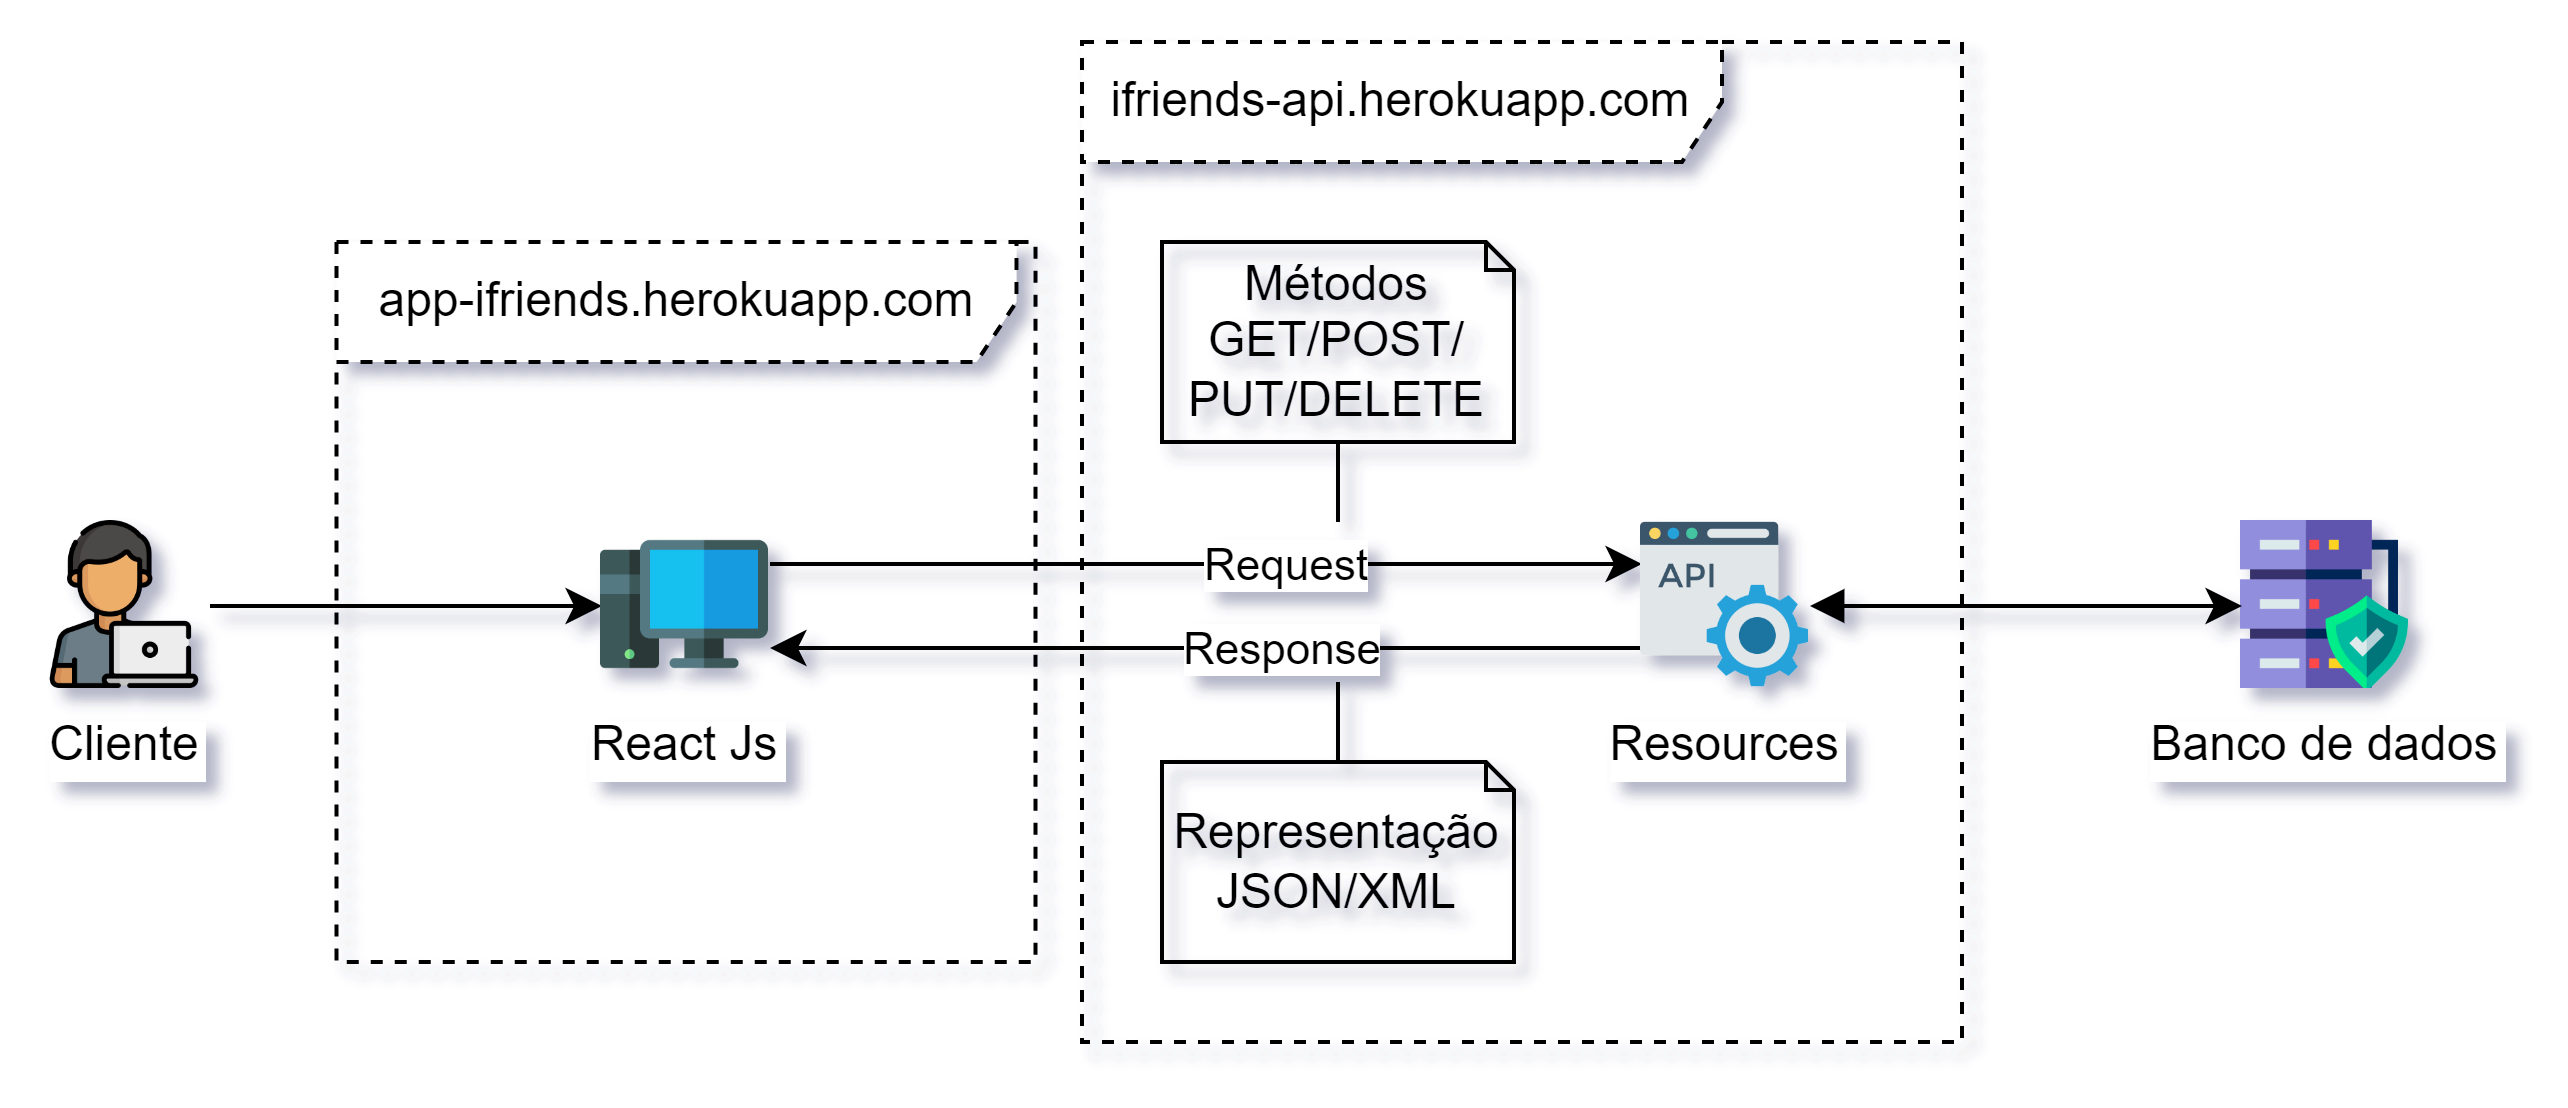
\includegraphics[width=1.0\textwidth]{anexos/Imagens_Diagramas/Arquitetura-Rest-API.png}
\fonte{Os autores.}
\end{figure}

Quanto ao banco de dados, será utilizado o \gls{postegreSQL}: um \acs{sgbd} popular de \acs{sql}, que serve para executar comandos no banco, como consultas, e alterações nos dados ou na estrutura.


Para hospedar a aplicação, será utilizado o \gls{heroku}, o qual é uma plataforma de nuvem que suporta diversas linguagens, que permite a implantação, escalonamento e gerenciamento do sistema.

Como inspiração para o sistema, será estudada sobre a plataforma \textit{Scoold}, a qual é uma aplicação  Web de código aberto de perguntas em respostas, inspirada no \textit{Stack Overflow}. Ela usa de base as mesmas tecnologias do projeto, tendo isso em vista, no caso da inviabilidade de seu uso, pode ser reaproveitado ideias implementadas nessa plataforma no seu código-fonte.

\subsection{Ferramentas de apoio}

Nesta seção serão especificados as ferramentas a serem utilizadas para a estruturação do sistema  Web.

\begin{itemize}
\item \textbf{Notion}: Foi escolhido como plataforma de organização de projetos, pois este possui métodos de gerenciamento de equipe, fornecendo uma interface para vários desenvolvedores trabalharem utilizando o quadro de kanban, assim como o compartilhamento de arquivos, vídeos e artigos; permitindo também notificações via e-mail sobre atualizações do projeto e de reuniões marcadas, por exemplo. 
    
\item \textbf{Discord}: Plataforma de comunicação online escolhida pela equipe, por ser a mais utilizada e conhecida entre os mesmos. Nela é possível criar servidores privados para compartilhar informações e realizar reuniões sobre o projeto.
    
\item \textbf{Overleaf}: Para a preparação do documento de visão, será usado o \LaTeX, visto que este possui comando de padronização para documentos acadêmicos, facilitando a sua construção, juntamente, com editor Overleaf que oferece um ambiente compartilhado entre os membros da equipe. 
    
\item \textbf{Figma}: Na parte de modelagem do sistema e elaboração ideias de soluções de problemas, escolheu-se o Figma, visto que é uma ferramenta gratuita que possui diversas opções de edição.
    
\item \textbf{Visual Studio Code}: A \acs{ide} escolhida para realizar a edição de código-fonte na parte \textsl{\gls{front-end}} do sistema, por razões de ser um recurso da atualidade com possibilidades de várias adaptações de ambiente, principalmente as nossas tecnologias escolhidas.

\item \textbf{Eclipse}: A \acs{ide} escolhida para realizar a edição de código-fonte na parte \textsl{\gls{back-end}}, por motivo de facilidade que o ambiente de desenvolvimento proporciona para rodar aplicações com Java e, também, seus recursos que fazem a integração com o banco de dados.
\end{itemize}



%---------------------------------------------------------------------------------------

%%%%%%%%%%%%%%%%%%%%%%%%%%%%%%%%%%%%%%%%
\section{Métodos de gestão e desenvolvimento}

Tendo em vista a organização do projeto \gls{ifriends}, a equipe escolheu utilizar os princípios e valores do Manifesto Ágil como norteadores nos seus processos de planejamento, modelagem e desenvolvimento do projeto. Deste modo, elencou-se  o \gls{framework} Scrum como metodologia ágil que irá servir como referência para o trabalho da Bunka Bytes.

\subsection{Metodologia ágil: Scrum} 
Segundo \citeonline{ambler2004modelagem}, o termo “metodologias ágeis” surgiu em fevereiro de 2001, quando  especialistas em processos de engenharia de \textsl{software} se reuniram e estabeleceram princípios comuns entre todas as metodologias, criando a Aliança Ágil e o estabelecimento do ``Manifesto Ágil'' \textsl{(Agile Manifesto)}.

O termo metodologia ágil consiste na otimização do tempo para a realização de determinado projeto, visando a rapidez na entrega e na qualidade do mesmo, surgindo assim, como uma resposta mais leve, mais assertiva e menos custosa em relação aos métodos pesados que eram utilizados para a construção de sistemas. Nas metodologias ágeis, os processos, as ferramentas, as documentações, as negociações e os planejamentos, possuem prioridade secundária, pois os indivíduos e suas interações são considerados essências e indispensáveis \cite{sganderla2016aprimorando}.

Para isso, o manifesto determina quatro valores principais, sendo eles: o enfoque nos indivíduos e nas interações, e não nos processos ou algoritmos; a adaptação e maior flexibilidade a novos fatores decorrentes do desenvolvimento do projeto; o foco na funcionalidade do sistema e na documentação mais simples e objetiva, e por último, a preferência por um ambiente de trabalho mais colaborativo e menos burocrático  \cite{sganderla2016aprimorando}. 

Segundo \citeonline{cruz:2018}, o Scrum pode ser definido como ``um \textsl{\gls{framework}} para desenvolver e manter produtos complexos que também pode ser utilizado no gerenciamento ágil de projetos que se destinam também à criação de produtos''. Neste caso, sabida a escolha da utilização de uma metodologia ágil para o gerenciamento do presente projeto, foi decidido aplicá-la com base no Scrum e suas especificações, porém, como a finalidade do trabalho é acadêmica, resolveu-se adaptar algumas de suas características para que a metodologia pudesse ser implementada como uma referência na organização e gestão do projeto. Estas, por conseguinte, serão explicitadas mais a frente, conforme apresentadas as particularidades do \textsl{\gls{framework}}.

Dentre as principais características do Scrum, está a divisão do desenvolvimento em ciclos repetitivos e curtos, permitindo modificações, adaptações e correções no produto de forma iterativa e incremental, o que, segundo \citeonline{cruz:2018} permite encontrar desvios mais rápido e com menos impacto. \citeonline{cruz:2018} explica que para que os processos sejam otimizados de tal forma, o Scrum possui ainda três pilares de sustentação: transparência, a inspeção e a adaptação.


Além dos pilares da metodologia, há cinco valores importantes para sua construção e prática durante um projeto: coragem, foco, comprometimento, respeito e abertura.  De acordo com \citeonline{cruz:2018} os valores do Scrum são responsáveis por reforçar os princípios do manifesto ágil, principalmente considerando o comportamento e as pessoas maiores do que os processos e ferramentas. 

%--------------------------------------------------------
\subsubsection{O quadro de kanban}

Segundo \citeonline{peinado2007compreendendo}, o nome Kanban vem do japonês ``cartão'' e a sua origem deu-se pela seguinte razão:

\begin{citacao}
Este nome surgiu em razão do sistema de controle visual dos estoques de materiais, pois são frequentemente utilizados cartões para representar os contentores cheios ou vazios, estes cartões são retirados ou colocados em um quadro à medida que o material é utilizado, ou reposto
\cite{peinado2007compreendendo}.
\end{citacao}
%%%%%%%%%%%%%%%%%%%%%%%%%%%
E através da implantação realizada por \citeonline{silva2012beneficios}, devido aos problemas e necessidades encontrados ao longo dos \textsl{sprints}, houve a criação de um processo ágil, baseado nas práticas do Scrum com características do Kanban:

\begin{citacao}
As tarefas ou itens de trabalho foram representadas através de cartões (do inglês \textsl{post-its}) fixados em um quadro (do inglês \textsl{cardwall}). 
Esse quadro, por sua vez, era dividido em colunas que representavam as fases do fluxo de trabalho (do inglês \textsl{workflow}) da equipe. 
As tarefas eram distribuídas sequencialmente nas colunas à medida que avançavam no fluxo de trabalho \cite{silva2012beneficios}.
\end{citacao}

No projeto  a implementação do kanban foi similar, porém todo o esquema presencial foi adaptado ao quadro remoto. Para conciliar a participação continua da equipe, a ferramenta \textsl{Notion} é utilizada como auxiliar aos processos de organização, onde também foi possível criar o quadro de kanban do projeto. 

O quadro de kanban usado pela equipe Bunka Bytes, responsável pelo projeto apresenta 5 colunas, nas quais são representadas visualmente em qual estagio a tarefa se encontra, as colunas se classificam como ``para fazer'', ``planejamento'', ``em andamento'', ``para revisar'' e ``feito''. E por ``cartões virtuais'' são colocadas as tarefas no quadro.

Foi decidido utilizar uma classificação em ordem de prioridade para cada tarefa, podendo ser "alta", representada pela cor vermelha, ``média'', representada pela cor laranja, e ``baixa'' representada pela cor verde, tais prioridades são atribuídas às tarefas assim que a \textsl{sprint} é definida.


De maneira geral, o uso do quadro de kanban é beneficial ao projeto, já que através de sua aplicação a equipe consegue conciliar de maneira clara e precisa as tarefas compartilhadas. A utilização do quadro remotamente, faz com que a equipe possa ainda acessá-lo de qualquer lugar, facilitando o processo de transparência dos itens e faz com que todos tenham em usas mão as atividades a serem feitas, podendo ajustá-las no momento em que preferirem. 

%------------------------------------------------



\subsection{Gestão da equipe}
A equipe Scrum é composta por três papéis: o \textsl{Scrum Master}, o \textsl{Product Owner} e o Time de Desenvolvimento:

\begin{citacao}

O primeiro, chamado \textsl{Scrum Master}, é considerado o responsável por garantir que o Scrum seja entendido e aplicado, para que o Time Scrum esteja aderindo os valores, as práticas e as regras do Scrum, e, portanto, trabalha como um líder ou técnico da equipe. Já o \textsl{Product Owner}, é o principal responsável pelo gerenciamento do \textsl{backlog} do produto, por garantir o valor do trabalho realizado pelo Time, e pela satisfação e atendimento das necessidades do cliente. O Time de Desenvolvimento, por outro lado, é responsável por executar o desenvolvimento e transformar o \textsl{backlog} do produto em incrementos de funcionalidades, criando um sistema pronto que possa ser entregue ao cliente \cite{cruz:2018}.

\end{citacao}

Portanto, para fins de organização, o Time de Desenvolvimento poderá ser dividido em subequipes, sendo elas: desenvolvimento ( \textsl{\gls{front-end}} e \textsl{\gls{back-end}}), design e documentação, e mídias. Nelas, estão inclusas as funções de programadores \textsl{\gls{front-end}} e \textsl{\gls{back-end}}, divididas entre os integrantes Jamilli Vitória Gioielli, José Roberto Claudinho Ferreira e Kaiky Matsumoto Silva; sendo a Jamilli responsável por supervisionar o \textsl{\gls{front-end}} da aplicação, e o José (que também auxiliará no \textsl{\gls{front-end}}) juntamente com o Kaiky pelo \textsl{\gls{back-end}} - que também inclui a administração do banco de dados. 

Além dessas, as outras duas subequipes foram dividias entre as integrantes Anaí Villca Rojas, responsável  por supervisionar o design de experiência/interface de usuário; e Julia Romualdo Pereira, responsável pelo gerenciamento da documentação e das mídias do projeto (como o canal no \gls{youtube} e as postagens no Blog). 

 De todo modo, a documentação e as mídias do projeto deverão ser revisadas, obrigatoriamente, por todo o time, de modo a manter um conhecimento sobre a aplicação melhormente distribuída. Entretanto, precisa-se compreender que a modelagem de dados e a elicitação de requisitos da aplicação serão feitas com o auxílio de todos os integrantes, visto que são partes de extrema importância para que a compreensão de todos sobre o cenário corresponda com o objetivo principal pretendido. No \autoref{distribuicao_tarefas}, é possível observar uma relação das supervisões dos integrantes em cada área do projeto. 

%%%%inserir tabela de relação das tarefas dos integrantes
\begin{quadro}[htb]
\centering
\ABNTEXfontereduzida
\caption{Distribuição de tarefas}
\label{distribuicao_tarefas}
\resizebox{\linewidth}{!}{

\begin{tabular}{|l|c|c|c|c|}
\hline

\thead{Responsável} & \thead{Front-end} & 
\thead{Back-end}  & \thead{Documentação e Mídias} & \thead{Design}\\
\hline
Anaí &    &    & \circlemark & \circlemark \\
\hline
Jamilli & \circlemark &  &  & \circlemark \\
\hline
José & \circlemark & \circlemark &  &   \\
\hline
Julia &  &  &  \circlemark &  \\
\hline
Kaiky & & \circlemark &  &  \\
\hline


\end{tabular}}\legend {Fonte: Os autores.}
\end{quadro}
\FloatBarrier 

Entretanto, é importante salientar que as funções atribuídas a cada um não são exclusivas e podem variar conforme a necessidade de entrega do projeto. As subequipes são de responsabilidade de todos os integrantes e apenas foram divididas assim para fins de organização das tarefas do projeto. Levando isso em consideração, as funções de \textsl{Scrum Master ou Iteration Manager} e \textsl{Product Owner} foram adaptadas, ainda que não seja o ideal na metodologia ágil, para um único papel, representado pela integrante Jamilli Vitória Gioielli. Porém, vale ressaltar ainda que, nesse modelo escolhido, toda a equipe é responsável pela inspeção dos processos do projeto, e não somente o \textsl{Scrum Master ou Iteration Manager}:

\begin{citacao}

O Time deve ser multidisciplinar e multifuncional, possuindo todo o conhecimento necessário para criar um incremento no trabalho. [...] Não há títulos no Time, e não há exceção a esta regra. Não deve existir distinção de cargos ou funções, títulos ou senioridades, e muito menos áreas determinadas ou específicas de atuação. No Scrum todos os integrantes do Time são conhecidos como “desenvolvedores”.

Individualmente os integrantes do Time de Desenvolvimento podem ter habilidades específicas, mas, independentemente disso, a responsabilidade a respeito de uma entrega continua sendo do Time de Desenvolvimento como um todo \cite{cruz:2018}.

\end{citacao}

Para organizar a produtividade continua de desenvolvimento do projeto, buscando seguir uma das vertentes propostas na metodologia ágil de entregas semanais, a equipe criou um cronograma de entregas por aula baseado a partir do plano de ensino da disciplina disponibilizado pelos orientadores, ou seja, a equipe busca realizar durante a semana a atividade proposta para a aula seguinte para aproveitar o tempo em sala de aula validando o que foi realizado com os orientadores. 

O cronograma de entrega semanal utilizado para o desenvolvimento do projeto \gls{ifriends} pode ser observado na \autoref{cronograma_desenvolvimento}.

\begin{figure}[htb]
\centering
\caption{Cronograma de Desenvolvimento Semanal}
\label{cronograma_desenvolvimento}
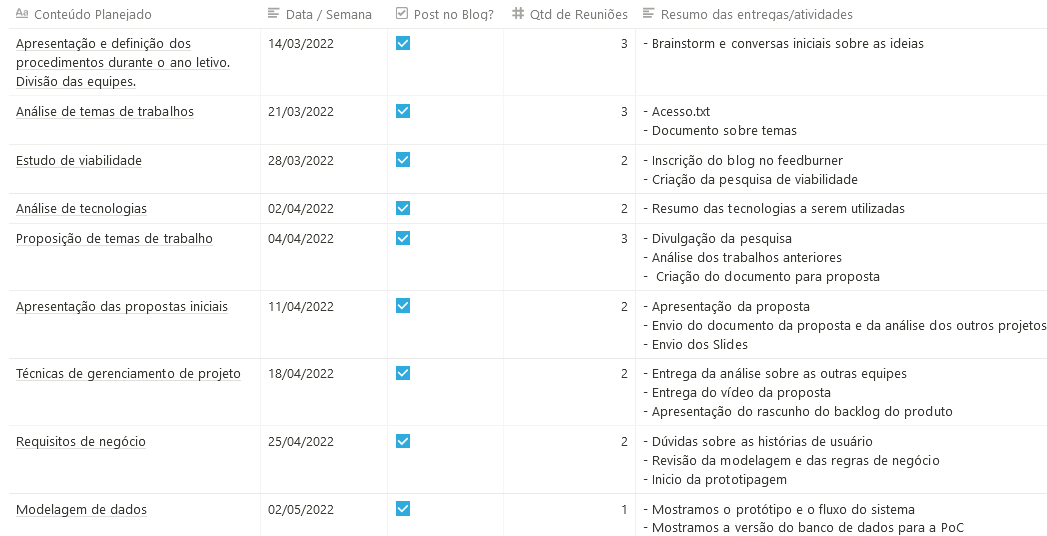
\includegraphics[width=1.0\textwidth]{anexos/Imagens_proposta/cronograma_desenvolvimento.png}
\fonte{Os autores.}
\end{figure}
\FloatBarrier

\subsection{Desenvolvimento: artefatos e eventos}

Tendo em vista a finalidade acadêmica do projeto, foi estipulado um valor mínimo de duas reuniões semanais dedicadas na construção do mesmo, levando em conta a organização individual de cada membro da equipe, além da priorização para que a tomada de decisões e planejamentos sejam feitas no dia das aulas da disciplina de \acs{pds}. Sobre os artefatos e eventos do Scrum, lista-se a seguir suas funcionalidades originais, descritos por \citeonline{cruz:2018}, e como serão adaptados:

\begin{itemize}
\item \textsl{Backlog}: é descrito como uma lista de todas as características, funções, tecnologias, melhorias e correções que constituem o produto a ser entregue. É também subdividido em ``do produto'', ``da versão de entrega'' e ``da \textsl{Sprint}'';

\item \textsl{Sprint}: originalmente pensada para durar um mês ou menos e possuir uma meta estabelecida com um objetivo claro, foi pensada 
para durar até duas semanas, já que as orientações da disciplina exigem que existam entregas frequentes, isto é, todas as semanas. Portanto, o ideal é que se dê início ao trabalho a ser entregue pelo menos uma semana antes de sua entrega;

\item \textsl{Time-boxed}: é esperado que o tempo estipulado para executar uma tarefa seja cumprido e que o trabalho proposto, seja realizado. Tendo em vista os curtos prazos,
também poderá ser adaptado conforme a entrega;

\item Planejamento da \textsl{Sprint}: ainda será utilizado para definir ``o que será feito'' e ``como'', porém, ao contrário das oito horas mínimas 
estipuladas, a equipe definiu um mínimo de duas horas para tal reunião, que poderá acontecer nas segundas-feiras, durante a aula de \acs{pds} ou aos finais de semana, logo após a finalização dos entregáveis;

\item Reuniões Diárias: não serão mantidas de maneira síncrona, visto que cada membro da equipe possui horários de disponibilidade diferentes. Porém, poderão ocorrer de forma assíncrona, de modo a compreender se existem impedimentos durante a execução das tarefas planejadas para a semana;

\item Revisão da \textsl{Sprint}: seu maior objetivo é a revisão do \textsl{Product Owner}, ou do cliente, em todos os itens concluídos pelo Time. Porém, 
não terá \textsl{Time-boxed} de quatro horas, visto que a aprovação dos professores orientadores (o cliente) pode ser mais rápida e acontecer durante a execução das tarefas. No entanto, o Time a realizará em todo final de entrega, para que os retornos dos professores levem em consideração o trabalho final;

\item Retrospectiva da \textsl{Sprint}: possui originalmente \textsl{Time-boxed} de até três horas e é feita para identificação 
de medidas de melhoria no processo do time que serão aplicadas na próxima \textsl{Sprint}. Foi escolhido adaptá-la para acontecer às terças-feiras, antes do início das aulas, para que as entregas feitas às segundas-feiras estejam frescas e o processo realizado pelo time possa ser melhor avaliado para a melhoria contínua.
\end{itemize}


Para a definição do \textsl{backlog} do produto, o Scrum conta com um recurso chamado histórias de usuário, que pode ser definido como: 

\begin{citacao}

História é uma descrição resumida, porém clara e objetiva, de alguma funcionalidade que deverá ser fornecida pelo produto a ser entregue, sempre do ponto de vista do usuário final. Uma história não é uma especificação completa da funcionalidade, mas uma promessa de discutir uma funcionalidade, ou, simplesmente, um lembrete de que a discussão já aconteceu. Um modelo simples de como escrever uma história seria: “Como um <tipo de usuário>, eu quero <um objetivo> para que <atenda a uma necessidade>.” \cite{cruz:2018}

\end{citacao}

Entretanto, vale ressaltar que as histórias de usuário do presente projeto serão montadas somente na parte de desenvolvimento, isto é, quando o produto começar a ser construído pelo Time Scrum e após os principais itens de \textsl{backlog} estarem descritos. Como ainda se encontra na fase de planejamento e modelagem, tal recurso ainda não foi acionado no projeto.

Outra ressalva diz respeito a utilização do \textsl{Scrum Poker} ou \textsl{Planning Poker Card}, que, segundo \citeonline{cruz:2018}, é definido como ``uma técnica que auxilia na estimativa de histórias e tarefas com base no consenso de todo o Time''. Para tanto, o Time utiliza um conjunto de cartas com valores representando os pontos ou horas por história. Sobre o funcionamento do \textsl{Planning Poker Card}:

\begin{citacao}

O seu uso é simples: o \textsl{Product Owner} ou um membro do Time apresenta a história, ou tarefa. Após uma breve discussão, cada um escolhe uma carta e a coloca virada sobre uma mesa, de forma que um não constate o valor da carta que o outro escolheu. Quando todos colocarem suas cartas, elas são desviradas para que todos vejam os valores.

Caso não haja consenso entre as cartas escolhidas, as diferenças são discutidas brevemente e uma nova rodada acontece, até que haja convergência e consenso.\cite{cruz:2018}

\end{citacao}

Para o presente projeto, no entanto, o \textsl{Planning Poker Card} será utilizado durante o processo de desenvolvimento do produto e após as histórias de usuário da \textsl{sprint} estarem bem descritas. Vale ressaltar que este processo é apenas para estimar o trabalho da equipe e pode variar conforme o andamento do projeto.
%%%%%%%%%%%%%%%%%%%%%%%%%%%%%%%%%%



%---------------------------------------------------------------------------------------



%--------------------------------------------------------------------------------
\chapter{Desenvolvimento}
  Baseando-se na conceituação de engenharia de \textsl{software} dada por \citeonline{SOMMERVILLE:2019}, neste capítulo é descrito o desenvolvimento do sistema, cujas etapas estão apoiadas em técnicas que vão desde sua especificação até sua evolução. Neste sentido, \citeonline{SOMMERVILLE:2019} destaca quatro etapas como fundamentais para os processos de \textsl{software}, sendo elas sequenciadas em: especificação, desenvolvimento, validação e evolução. As etapas correspondentes a este capítulo consistem na definição, junto as suas restrições, e na projeção do sistema para ser programado - isto é, a especificação e o desenvolvimento.
  
  Desse modo, as especificações descritas no capítulo estão separadas em: análise de requisitos, regras do negócio, modelagem do sistema e prototipação.

%------------------------------------------------------


%------------------------------------------------------
\section{Análise de Requisitos}
Segundo \citeonline{machado2018analise}, ao definir as características de um requisito, é preciso salientar que não são dependentes da tecnologia empregada, visto que suas especificações estão contidas no campo do cumprimento das necessidades do usuário. Dessa forma,  \citeonline{machado2018analise} define os requisitos como ``objetivos ou restrições estabelecidas por clientes e usuários do sistema que definem suas diversas propriedades''.

Assim, tanto \citeonline{machado2018analise} como \citeonline{SOMMERVILLE:2019} concordam que a fase de definição de requisitos, a chamada engenharia de requisitos, é essencial para a tomada de decisões sobre os passos para adquirir ou desenvolver o sistema. Por outro lado, Sommerville ainda acrescenta sobre a necessidade de mudança durante o desenvolvimento:

\begin{citacao}
Naturalmente, são feitas mudanças subsequentes nos requisitos de usuário, que podem ser ampliados para requisitos de sistema mais detalhados. Às vezes, pode-se utilizar uma abordagem ágil para elicitar simultaneamente os requisitos à medida que o sistema é desenvolvido, a fim de acrescentar detalhes e refinar os requisitos de usuário \cite{SOMMERVILLE:2019}.
\end{citacao}

Tendo tais definições em vista, as próximas seções visam apresentar os requisitos funcionais e não funcionais, e as regras do negócio característicos do projeto tratado neste documento. Para representar os requisitos funcionais e os requisitos não funcionais se usou as histórias de usuário. Foi com base na utilização da abordagem ágil no projeto (mais especificada na seção 3), que se definiu três prioridades principais: alta, média e baixa. 

A prioridade alta é aquela correspondente aos requisitos obrigatórios para o funcionamento do sistema, isto é, aqueles que caso faltem, o sistema em si não existe; já na prioridade média, por exemplo, são característicos aqueles desejáveis, ou seja, são importantes para o sistema, mas não interferem diretamente numa mudança brusca de seu comportamento. Desse modo, os requisitos de prioridade baixa, são tidos como opcionais, aqueles que podem entrar no sistema eventualmente, mas que, numa fila de produção, não serão feitos antes dos demais. Vale ressaltar, por conseguinte, que tais decisões dependem da negociação entre os envolvidos no projeto e do método de produção utilizado, como descrevem \citeonline{vazquezsimoes:2016}. Os autores ainda completam, dizendo:


\begin{citacao}
A priorização tem como função assegurar que os recursos do projeto sejam focados nos itens mais relevantes. Daí a importância de, na especificação, diferenciar cada requisito em termos de importância, dentre dezenas ou centenas de outros requisitos.

A responsabilidade por definir a prioridade do requisito deveria ser da parte interessada, facilitada pelo gerente de projetos \cite{vazquezsimoes:2016}.
\end{citacao}

\subsection{Histórias de Usuário}
Segundo \citeonline{cruz:2018} as histórias de usuário se caracterizam como uma descrição resumida, clara e objetiva de uma funcionalidade fornecida pelo produto a ser entregue, visando o ponto de vista final do usuário. Ainda segundo o autor para uma história ser tida como completa, ela deve possuir uma descrição objetiva e critérios de aceitação, esses critérios representam o que ela precisa fazer para ser considerada válida.

No projeto, a equipe aproveitou as histórias de usuário para representar os requisitos funcionais e não funcionais, dessa forma os requisitos funcionais podem ser identificados a partir do nome das histórias, e o não funcionais por meio dos critérios de aceitação definidos para tais. Além disso, considerando a entrega da \acs{POC}, as histórias foram separadas conforme a elaboração dos dois épicos preparados para esta entrega, sendo elas a gestão de perguntas e a gestão de respostas.

Todas as histórias apresentam sete componentes: o seu nome, a sua descrição, seus critérios de aceitação, o épico a qual pertence, a pontuação que ela recebeu no \textsl{planning poker}, a estimativa de tamanho conforme a sua pontuação e a sua prioridade conforme o seu tamanho e pontuação.

%%%%%%%  História - Manter uma pergunta %%%%%%% 
\def\arraystretch{2}
\begin{quadro}[htb]
\centering
\ABNTEXfontereduzida
\caption[História: Manter uma pergunta]{História: Manter uma pergunta}
\resizebox{\linewidth}{!}{
\begin{tabular}{|p{6.5cm}|c|c|c|c|}
\hline
\thead{Descrição} & \thead{Épico} & \thead{Pontuação} & \thead{Tamanho} & \thead{Prioridade}\\
\hline

Como aluno, eu gostaria de manter uma pergunta na comunidade para retirar uma dúvida & Gestão de Perguntas & 13 & Grande & ALTA \\ \hline

\end{tabular}}\legend{Fonte: Os autores}
\end{quadro}
\FloatBarrier 

Para esta história de usuário foram definidos os seguintes itens como critérios de aceitação:

\begin{itemize}
\item Mostrar ``como fazer uma boa pergunta'';
\item O usuário deve conseguir somente criar e remover uma pergunta da visualização;
\item O usuário deve conseguir fechar o espaço de resposta para a pergunta;
\end{itemize}

%%%%%%% História - Buscar Perguntas %%%%%%% 
\def\arraystretch{2}
\begin{quadro}[htb]
\centering
\ABNTEXfontereduzida
\caption[História: Buscar perguntas]{História: Buscar perguntas}
\resizebox{\linewidth}{!}{
\begin{tabular}{|p{6.5cm}|c|c|c|c|}
\hline
\thead{Descrição} & \thead{Épico} & \thead{Pontuação} & \thead{Tamanho} & \thead{Prioridade}\\
\hline

Como aluno, eu gostaria de buscar perguntas feitas para que possa consultar uma pergunta específica & Gestão de Perguntas & 2 & Pequena & Média \\ \hline

\end{tabular}}\legend{Fonte: Os autores}
\end{quadro}
\FloatBarrier 

Para esta história de usuário foram definidos os seguintes itens como critérios de aceitação:

\begin{itemize}
\item O usuário precisa informar total ou parcialmente o título da pergunta desejada;
\item As perguntas serão exibidas conforme as informações passadas, podendo ser semelhantes parcial ou totalmente;
\end{itemize}

%%%%%%% História - Curtir uma pergunta %%%%%%% 
\def\arraystretch{2}
\begin{quadro}[htb]
\centering
\ABNTEXfontereduzida
\caption[História: Curtir uma pergunta]{História: Curtir uma pergunta}
\resizebox{\linewidth}{!}{
\begin{tabular}{|p{6.5cm}|c|c|c|c|}
\hline
\thead{Descrição} & \thead{Épico} & \thead{Pontuação} & \thead{Tamanho} & \thead{Prioridade}\\
\hline

Como aluno, eu gostaria de votar em uma pergunta para indicar se ela me foi útil ou não. & Gestão de Perguntas & 2 & Pequena & Alta \\ \hline

\end{tabular}}\legend{Fonte: Os autores}
\end{quadro}
\FloatBarrier 

Para esta história de usuário foram definidos os seguintes itens como critérios de aceitação:

\begin{itemize}
\item Um usuário só poderá votar uma única vez;
\item Cada voto equivale a um ponto;
\item Soma dos pontos por pergunta deve ser exibida;
\end{itemize}

%%%%%%% História - Manter uma resposta %%%%%%% 
\def\arraystretch{2}
\begin{quadro}[htb]
\centering
\ABNTEXfontereduzida
\caption[História: Manter uma resposta]{História: Manter uma resposta}
\resizebox{\linewidth}{!}{
\begin{tabular}{|p{6.5cm}|c|c|c|c|}
\hline
\thead{Descrição} & \thead{Épico} & \thead{Pontuação} & \thead{Tamanho} & \thead{Prioridade}\\
\hline

Como aluno, eu gostaria de manter uma resposta para retirar uma dúvida de um colega. & Gestão de Respostas & 5 & Média & Alta \\ \hline

\end{tabular}}\legend{Fonte: Os autores}
\end{quadro}
\FloatBarrier 

Para esta história de usuário foram definidos os seguintes itens como critérios de aceitação:

\begin{itemize}
\item As respostas mais curtidas devem ser exibidas antes das demais;
\item O usuário deve conseguir somente criar e deletar uma resposta;
\item Todas as respostas devem ser exibidas sem exceção;
\end{itemize}

%%%%%%% História - Curtir uma resposta %%%%%%% 
\def\arraystretch{2}
\begin{quadro}[htb]
\centering
\ABNTEXfontereduzida
\caption[História: Curtir uma resposta]{História: Curtir uma resposta}
\resizebox{\linewidth}{!}{
\begin{tabular}{|p{6.5cm}|c|c|c|c|}
\hline
\thead{Descrição} & \thead{Épico} & \thead{Pontuação} & \thead{Tamanho} & \thead{Prioridade}\\
\hline

Como aluno, eu gostaria de curtir uma resposta para indicar se ela me foi útil ou não. & Gestão de Respostas & 1 & Pequena & Alta \\ \hline

\end{tabular}}\legend{Fonte: Os autores}
\end{quadro}
\FloatBarrier 

Para esta história de usuário foram definidos os seguintes itens como critérios de aceitação:

\begin{itemize}
\item Um usuário só poderá curtir uma única vez;
\item Cada curtida equivale a um ponto;
\item Soma das curtidas por pergunta deve ser exibida;
\end{itemize}


\subsection{Regras de Negócio}
Regras de negócio são requisitos de domínio de aplicação tratado no desenvolvimento de um sistema, isso significa, as declarações sobre como determinada empresa faz negócio. É a partir dessas regras que se define como o negócio funciona e quais são suas especificações, além da sua importância para o desenvolvimento de um sistema, pois, auxiliam no controle dos processos, ajudam na tomada de decisões além de afetarem diretamente os requisitos funcionais, como descrevem \citeonline{dallavalle2000regras}. Dessa forma, o \autoref{regras negocio} lista as regras de negócio levantadas para o projeto \gls{ifriends}.

\def\arraystretch{2}
\begin{quadro}[thb]
\centering
\ABNTEXfontereduzida
\caption{Regras de Negócio}
\label{regras negocio}
\resizebox{\linewidth}{!}{
\begin{tabular}{|c|p{13cm}|}
\hline
\textbf{ID} & \textbf{Descrição} \\
\hline
\acs{RN}01 & Não serão permitidos usuários com os mesmos dados, ou seja, o sistema só permitirá a criação de uma conta por usuário \\
\hline
\acs{RN}02 & A fim de garantir a segurança de nossos usuários, o sistema deverá fazer uso de algumas diretrizes da Lei Marco Civil da Internet, lei n\textdegree 12.965/2014, que tem como objetivo estabelecer princípios, garantias, direitos e deveres para o uso da internet no Brasil. \\
\hline
\acs{RN}03 & Dentro do direito a exclusão, ao excluir seu perfil, o usuário deve ter ciência de que suas perguntas e respostas serão mantidas na comunidade, porém como parte de um usuário anônimo (exemplo: user12345678). \\
\hline
\acs{RN}04 & O usuário deve resumir seu problema dentro do título da pergunta. \\
\hline
\acs{RN}05 & O usuário deve descrever seu problema, informar de forma clara o que ele precisa. \\
\hline
\acs{RN}06 &  O usuário deve descrever qual cenário o colocou nessa situação, o que já tentou e qual seu objetivo final. \\
\hline
\acs{RN}07 &  Se necessário, se deve fazer uso de imagens a fim de explicando melhor o problema. \\
\hline
\acs{RN}08 & O usuário deve lembrar que podem haver respostas diferentes, portanto deve manter a mente aberta a novas sugestões. \\
\hline

\end{tabular}}\legend {Fonte: os autores}
\end{quadro}
\FloatBarrier 


\section{Modelagem}
Segundo \citeonline{SOMMERVILLE:2019}, a modelagem de sistemas é definida como ``um processo de desenvolvimento de modelos abstratos de um sistema, cada um apresentando uma visão diferente do mesmo''. Para isso, descreve também que são geralmente usadas notações gráficas baseadas nos tipos de diagrama em \acs{uml} durante o processo de engenharia de requisitos ``para ajudar a derivar os requisitos detalhados de um sistema; durante o processo [...]; e depois da implementação, para documentar a estrutura e operação do sistema'' \cite{SOMMERVILLE:2019}. 

\subsection{Diagrama de Casos de Uso}
De acordo com \citeonline{umlGuedes}, o diagrama de casos de uso \acs{uml} é descrito como:

\begin{citacao}
O diagrama de casos de uso [...] tem por objetivo apresentar uma visão externa geral das funcionalidades que o sistema deverá oferecer aos usuários, sem se preocupar com a questão de como tais funcionalidades serão implementadas. [...] É de grande auxílio para a identificação e compreensão dos requisitos do sistema, ajudando a especificar, visualizar e documentar as características, funções e serviços do sistema desejados pelo usuário \cite{umlGuedes}.
\end{citacao}

Logo, a \autoref{diagrama_CasosUso} representa os casos de uso do projeto de sistema \gls{ifriends}.

\begin{figure}[htb]
\centering
\caption{Diagrama de Casos de Uso}
\label{diagrama_CasosUso}
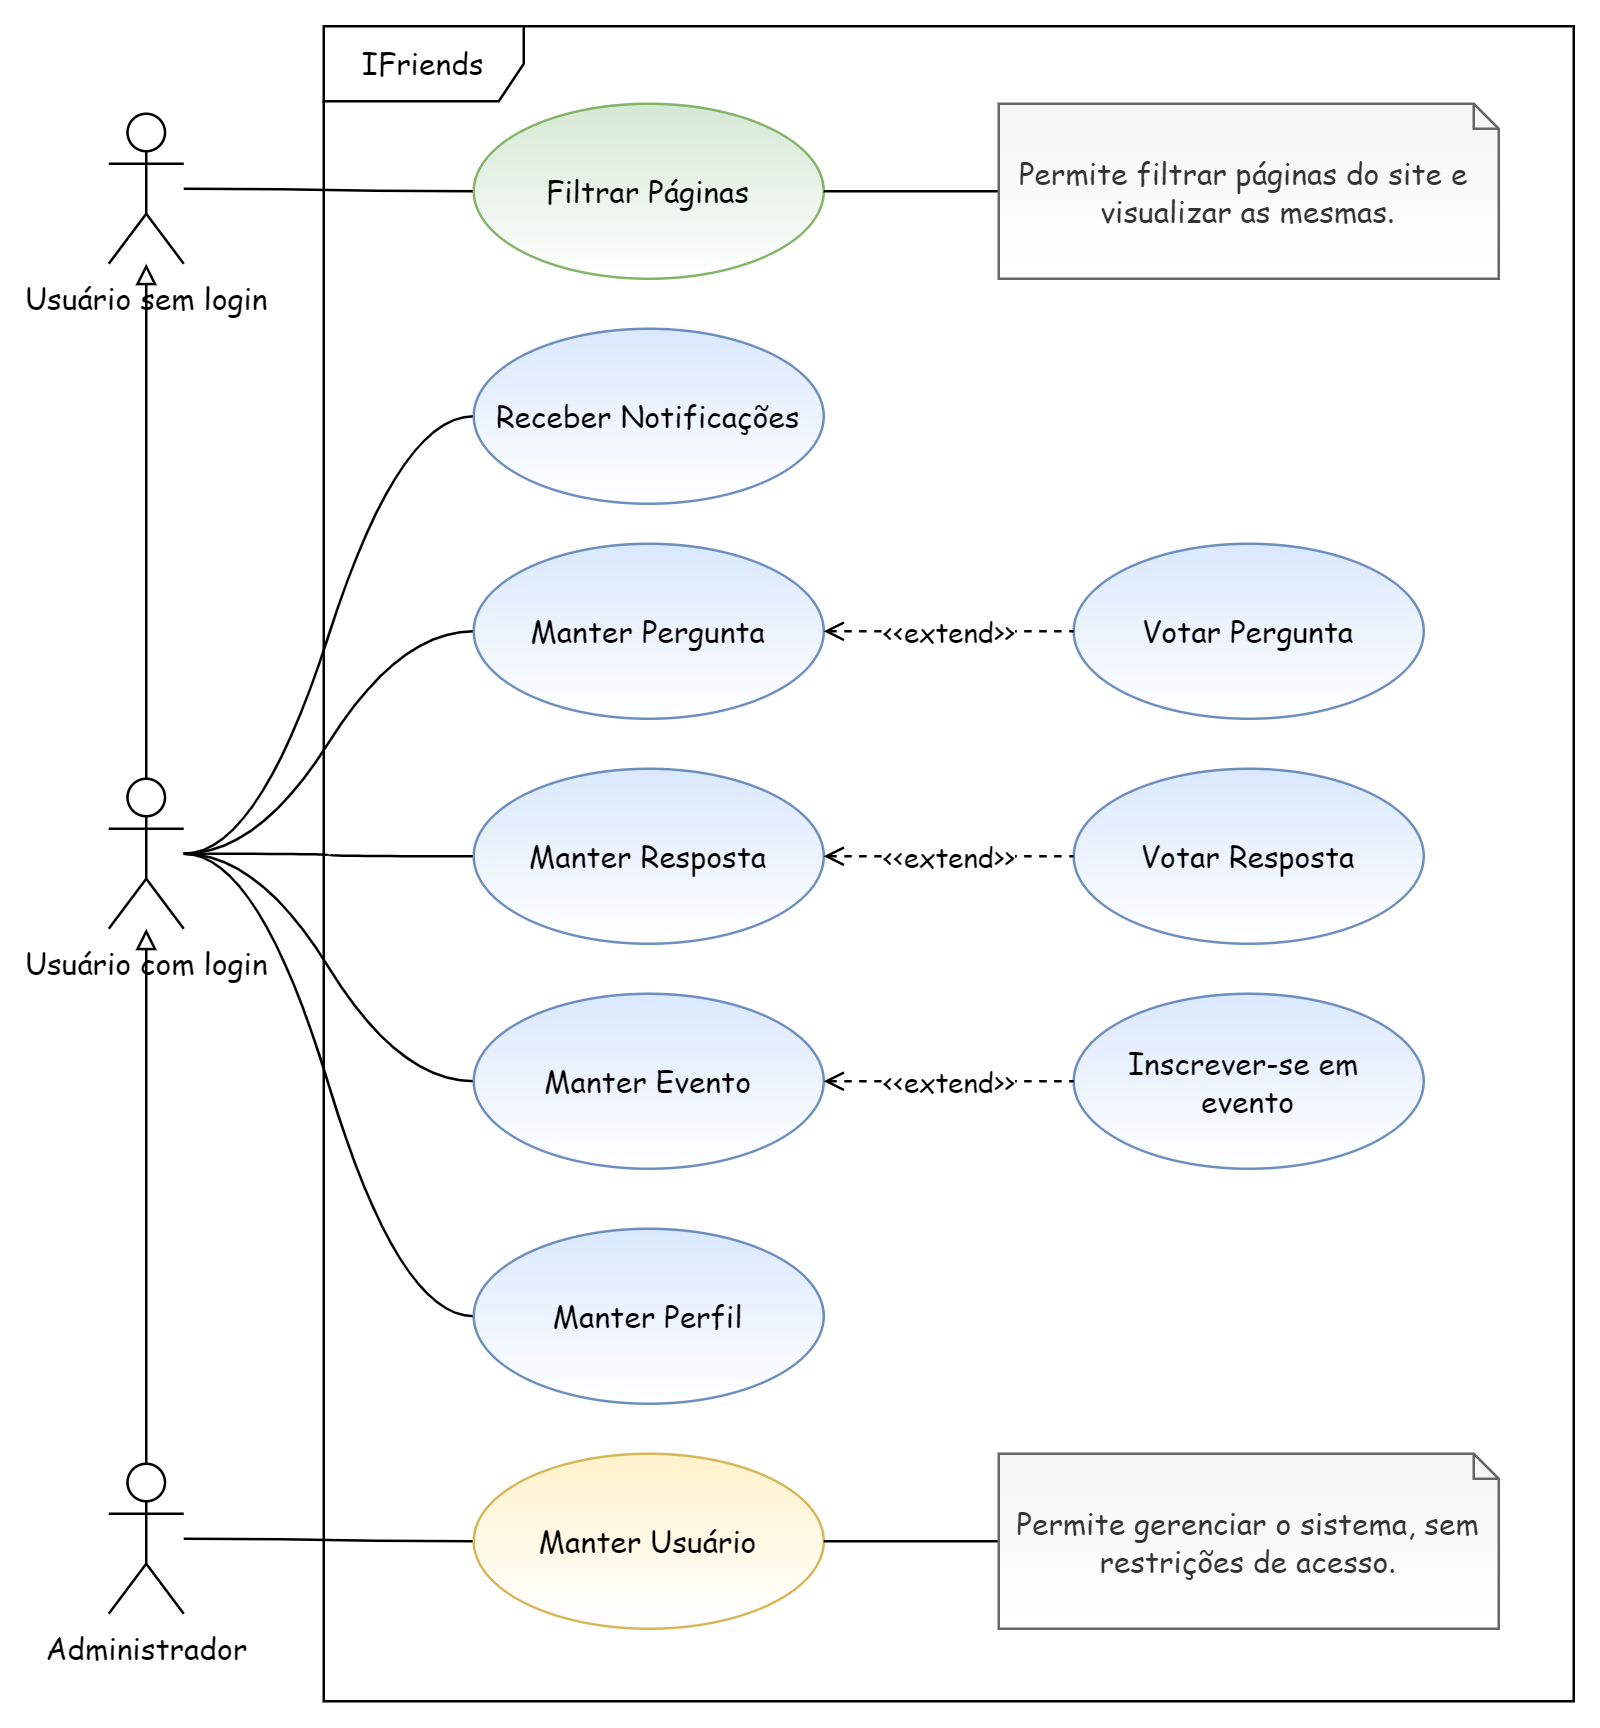
\includegraphics[width=1.0\textwidth]{anexos/Imagens_Diagramas/CasosDeUso_IFriends.png}
\fonte{Os autores.}
\end{figure}
\FloatBarrier


%\subsection{Diagrama de Classes}
% É necessário?

\subsection{Diagrama de Entidade e Relacionamento}

De acordo com \citeonline{leal2015linguagem}, a abordagem entidade-relacionamento é a técnica de modelagem de dados mais difundida e utilizada e representa a modelo conceitual do banco de dados. Nela, a estrutura do banco de dados é descrita como coleção de entidades, relacionamentos e representada graficamente por meio do Diagrama Entidade Relacionamento.

Através dele, é possível descrever um subconjunto do mundo real que será retratado no banco de dados com um alto nível de abstração. Além disso, o modelo Entidade Relacionamento é um modelo formal e caracteriza-se por ter uma grande capacidade semântica, o que garante que todos possam ter o mesmo entendimento \cite{leal2015linguagem}.

A \autoref{diagrama_EntidadeRelacionamento} representa o \ac{der} do projeto de sistema \gls{ifriends}.

\begin{figure}[htb]
\centering
\caption{Diagrama de Entidade e Relacionamento}
\label{diagrama_EntidadeRelacionamento}
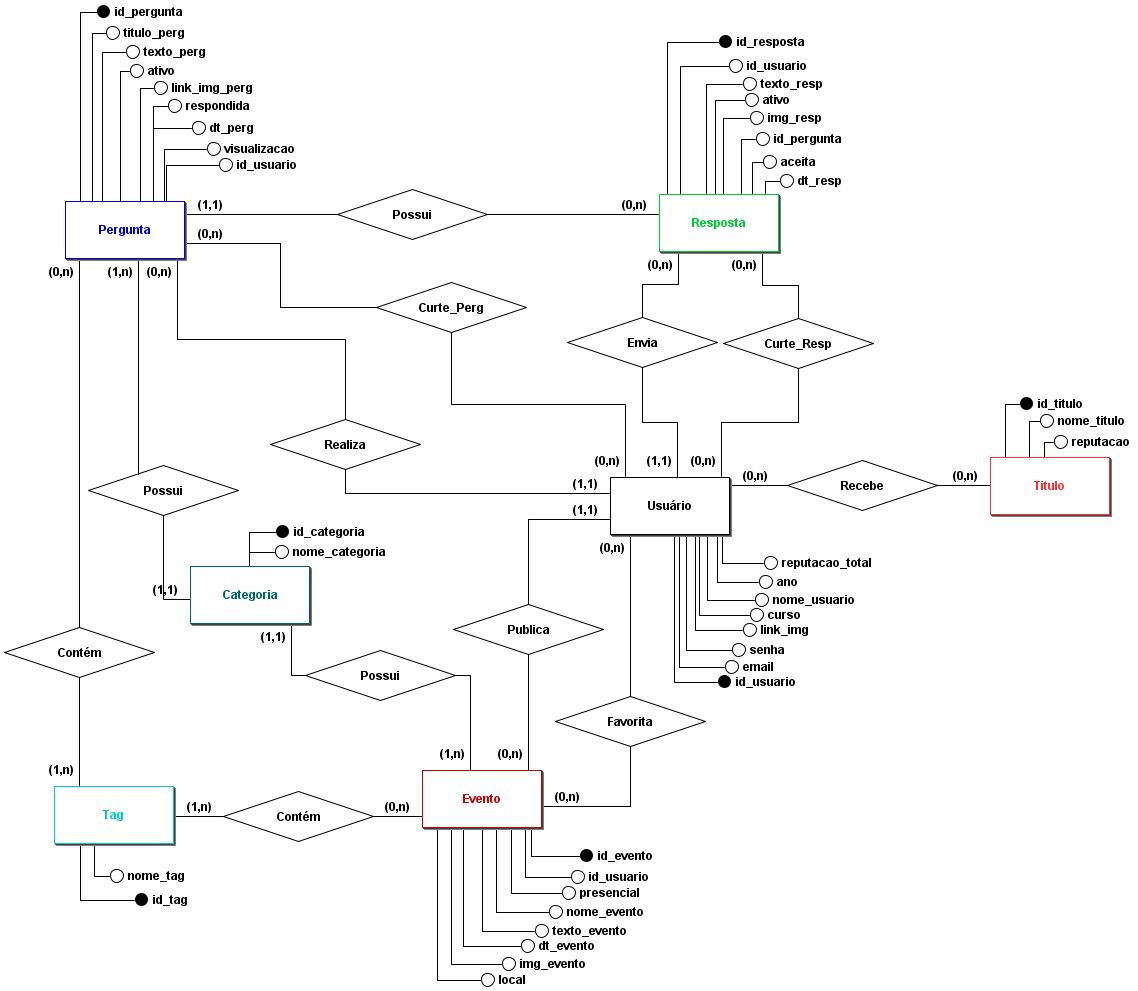
\includegraphics[width=1.0\textwidth]{anexos/Imagens_Diagramas/DER_IFriends.png}
\fonte{Os autores.}
\end{figure}
\FloatBarrier


\subsection{Diagrama de Tabelas Relacionais}

O Diagrama de Tabelas Relacionais \acs{dtr} representa o modelo lógico do Banco de Dados. Segundo \citeonline{utilidadepublica:201?}, através do modelo lógico é representado de maneira mais clara as entidades e os relacionamentos, pois considera algumas limitações e implementa recursos como adequação de padrão e nomenclatura, define as chaves primárias e estrangeiras, normalização, integridade referencial, entre outras.

Deste modo, a \autoref{diagrama_TabelasRelacionais} representa o \ac{dtr} do projeto de sistema \gls{ifriends}.

\begin{figure}[htb]
\centering
\caption{Diagrama de Tabelas Relacionais}
\label{diagrama_TabelasRelacionais}
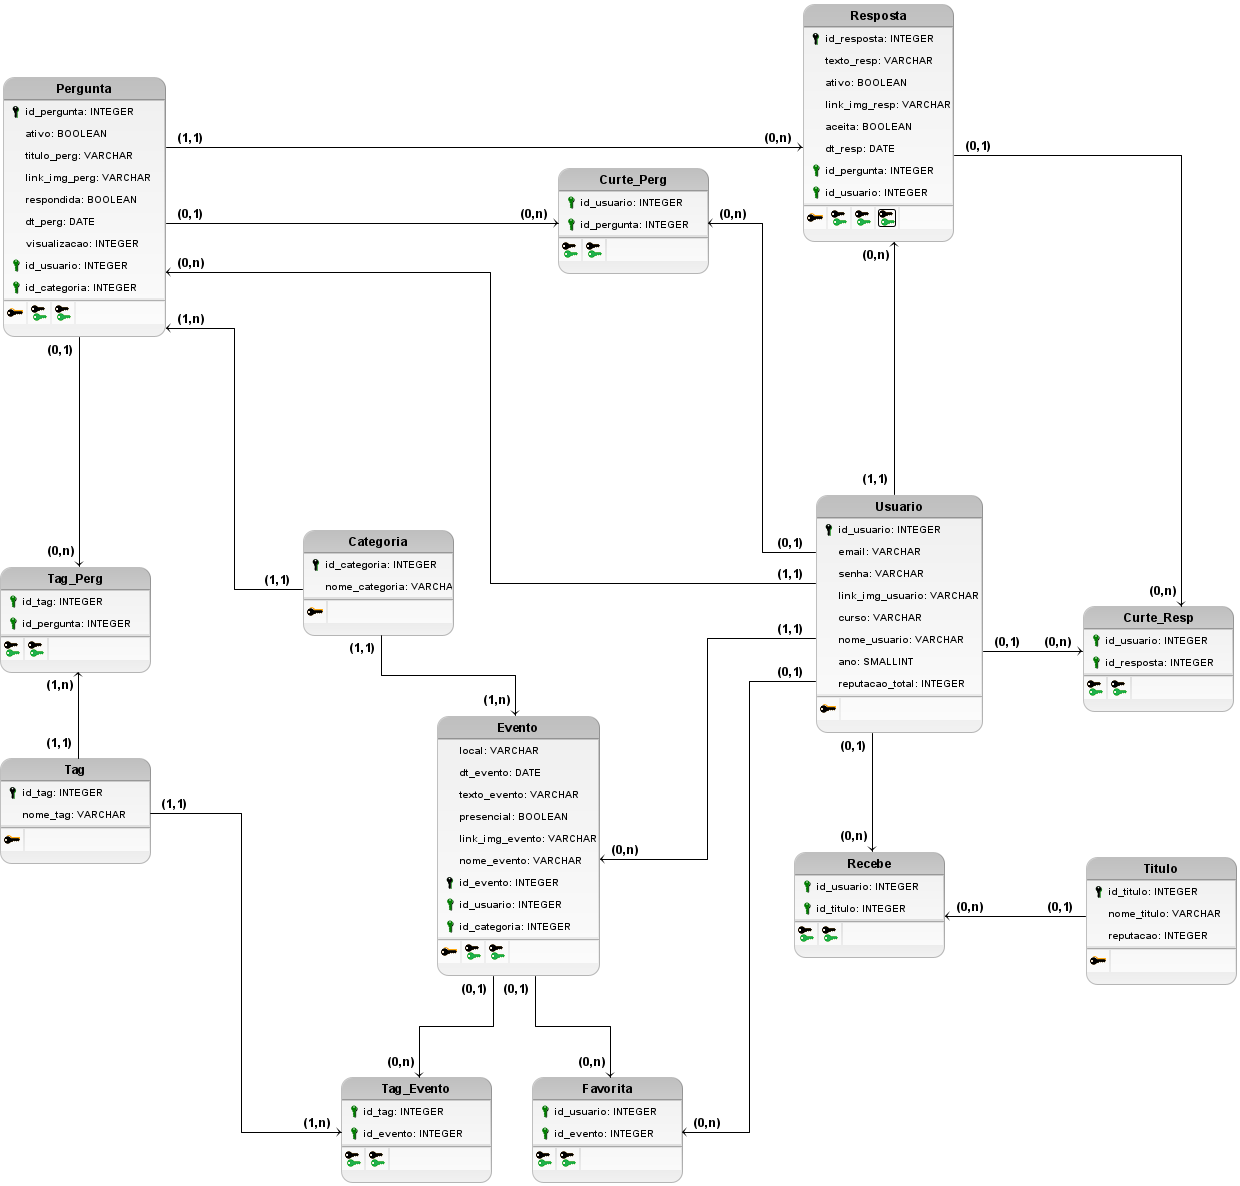
\includegraphics[width=0.9\textwidth]{anexos/Imagens_Diagramas/DTR_IFriends.png}
\fonte{Os autores.}
\end{figure}
\FloatBarrier

\subsection{Dicionário de Dados}

O Dicionário de dados é responsável por armazenar as informações de configuração do banco de dados e as estruturas que compõem suas respectivas tabelas. As estruturas definem os campos e suas propriedades \cite{alvesbanco}.

Conforme \citeonline{date2004introdução}, o Dicionário de dados é o lugar em que – dentre outras coisas – todos os diversos esquemas (externo, conceitual, interno) e todos os mapeamentos correspondentes são mantidos.

O Dicionário de dados contém os metadados, dados que explicam dados, com relação aos diversos objetos que são de interesse do próprio sistema. Exemplos desses objetos incluem índices, usuários, restrições de integridade, restrições de segurança, e assim por diante, informações que essenciais para que o sistema faça seu trabalho apropriadamente \cite{date2004introdução}.

De tal modo, abaixo encontram-se os quadros que representam o \ac{dd} das tabelas de banco de dados do projeto \gls{ifriends}.

%%%%%%%%% Tabela usuario
\def\arraystretch{1.5}

\begin{quadro}[htb]
\centering
\ABNTEXfontereduzida
\caption[Usuário]{Usuário.}
\begin{tabular}{|>{\Centering}m{3cm}|>{\Centering}m{1.75cm}|>{\Centering}m{1.6cm}|>{\Centering}m{1.15cm}|>{\Centering}m{1.25cm}|m{4.5cm}|}
\hline
\thead{Atributo} & \thead{Tipo} & \thead{Tamanho} & \thead{Nulo} & \thead{Chave} & \thead{Descrição}\\
\hline

id\_usuario & INT & 11 & N & PK & Chave primária do usuário \\ \hline
email & VARCHAR & 50 & N &  & E-mail institucional do usuário \\ \hline
senha & VARCHAR & 50 & N &  & Senha de acesso ao sistema \\ \hline
link\_img & TEXT &  & S &  & link da imagem de perfil \\ \hline
curso & VARCHAR & 50 & S &  & Curso atual \\ \hline
nome\_usuario & VARCHAR & 120 & N &  & Nome do usuário \\ \hline
ano & INT & 1 & S &  & Ano que o usuário cursa, ex.: 1\textdegree ano \\ \hline
reputacao\_total & INT & 11 & N  &  & Pontuação da reputação do usuário \\ \hline

\end{tabular}\legend{Fonte: Os autores}
\end{quadro}
\FloatBarrier 

%%%%%%%% Tabela usuario - pergunta
\def\arraystretch{1.5}

\begin{quadro}[htb]
\centering
\ABNTEXfontereduzida
\caption[Usuário\_Pergunta]{Usuário\_Pergunta.}
\label{quadro-dicionario-dados}
\begin{tabular}{|>{\Centering}m{3cm}|>{\Centering}m{1.75cm}|>{\Centering}m{1.6cm}|>{\Centering}m{1.15cm}|>{\Centering}m{1.25cm}|m{4.5cm}|}
\hline
\thead{Atributo} & \thead{Tipo} & \thead{Tamanho} & \thead{Nulo} & \thead{Chave} & \thead{Descrição}\\
\hline

id\_usuario & INT & 11 & N & FK & Chave estrangeira no usuário \\ \hline
id\_pergunta & INT & 11 & N & FK & Chave estrangeira na pergunta \\ \hline

\end{tabular}\legend{Fonte: Os autores}
\end{quadro}
\FloatBarrier 

%\clearpage

%usuario - resposta
\def\arraystretch{1.5}

\begin{quadro}[htb]
\centering
\ABNTEXfontereduzida
\caption[Usuário\_Resposta]{Usuário\_Resposta.}
\label{quadro-dicionario-dados}
\begin{tabular}{|>{\Centering}m{3cm}|>{\Centering}m{1.75cm}|>{\Centering}m{1.6cm}|>{\Centering}m{1.15cm}|>{\Centering}m{1.25cm}|m{4.5cm}|}
\hline
\thead{Atributo} & \thead{Tipo} & \thead{Tamanho} & \thead{Nulo} & \thead{Chave} & \thead{Descrição}\\
\hline

id\_usuario & INT & 11 & N & FK & Chave estrangeira no usuário \\ \hline
id\_resposta & INT & 11 & N & FK & Chave estrangeira na resposta \\ \hline

\end{tabular}\legend{Fonte: Os autores}
\end{quadro}
\FloatBarrier 

%usuario - Titulo
\def\arraystretch{1.5}

\begin{quadro}[htb]
\centering
\ABNTEXfontereduzida
\caption[Usuário\_Título]{Usuário\_Título.}
\label{quadro-dicionario-dados}
\begin{tabular}{|>{\Centering}m{3cm}|>{\Centering}m{1.75cm}|>{\Centering}m{1.6cm}|>{\Centering}m{1.15cm}|>{\Centering}m{1.25cm}|m{4.5cm}|}
\hline
\thead{Atributo} & \thead{Tipo} & \thead{Tamanho} & \thead{Nulo} & \thead{Chave} & \thead{Descrição}\\
\hline

id\_usuario & INT & 11 & N & FK & Chave estrangeira no usuário \\ \hline
id\_titulo & INT & 11 & N & FK & Chave estrangeira no titulo \\ \hline

\end{tabular}\legend{Fonte: Os autores}
\end{quadro}
\FloatBarrier 


%Titulo
\def\arraystretch{1.5}

\begin{quadro}[htb]
\centering
\ABNTEXfontereduzida
\caption[Título]{Título.}
\label{quadro-dicionario-dados}
\begin{tabular}{|>{\Centering}m{3cm}|>{\Centering}m{1.75cm}|>{\Centering}m{1.6cm}|>{\Centering}m{1.15cm}|>{\Centering}m{1.25cm}|m{4.5cm}|}
\hline
\thead{Atributo} & \thead{Tipo} & \thead{Tamanho} & \thead{Nulo} & \thead{Chave} & \thead{Descrição}\\
\hline

id\_titulo & INT & 11 & N & PK & Chave primária do título \\ \hline
nome\_titulo & VARCHAR & 50 & N &  & Nome do título \\ \hline
reputacao & INT & 11 & N & & Acumulo da pontuação \\\hline

\end{tabular}\legend{Fonte: Os autores}
\end{quadro}
\FloatBarrier 
%\clearpage

%Resposta
\def\arraystretch{1.5}

\begin{quadro}[htb]
\centering
\ABNTEXfontereduzida
\caption[Resposta]{Resposta.}
\label{quadro-dicionario-dados}
\begin{tabular}{|>{\Centering}m{3cm}|>{\Centering}m{1.75cm}|>{\Centering}m{1.6cm}|>{\Centering}m{1.15cm}|>{\Centering}m{1.25cm}|m{4.5cm}|}
\hline
\thead{Atributo} & \thead{Tipo} & \thead{Tamanho} & \thead{Nulo} & \thead{Chave} & \thead{Descrição}\\ \hline

id\_resposta & INT & 11 & N & PK & Chave primária da resposta \\ \hline
id\_usuario & INT & 11 & N & FK  & Chave estrangeira de usuário \\ \hline
id\_pergunta & INT & 11 & N & FK & Chave estrangeira de pergunta \\ \hline
texto\_resp & TEXT &  & N &  & Conteúdo da resposta \\ \hline
ativo & BOOLEAN & & N & & Resposta ativa ou não \\ \hline
img\_resp & TEXT & & S & & Imagem da resposta \\ \hline
aceita & BOOLEAN & & N & & Se a resposta foi aceita como solução válida para o autor da pergunta \\ \hline
dt\_resposta & DATE & 50 & N & & Data em que a resposta foi publicada \\ \hline

\end{tabular}\legend{Fonte: Os autores}
\end{quadro}
\FloatBarrier 

%Tag
\def\arraystretch{1.5}

\begin{quadro}[htb]
\centering
\ABNTEXfontereduzida
\caption[Tag]{Tag.}
\label{quadro-dicionario-dados}
\begin{tabular}{|>{\Centering}m{3cm}|>{\Centering}m{1.75cm}|>{\Centering}m{1.6cm}|>{\Centering}m{1.15cm}|>{\Centering}m{1.25cm}|m{4.5cm}|}
\hline
\thead{Atributo} & \thead{Tipo} & \thead{Tamanho} & \thead{Nulo} & \thead{Chave} & \thead{Descrição}\\
\hline

id\_tag & INT & 3 & N & PK & Chave primária da tag \\ \hline
nome\_tag & VARCHAR & 50 & N &  & Nome da tag \\ \hline

\end{tabular}\legend{Fonte: Os autores}
\end{quadro}
\FloatBarrier 
%\clearpage

%Pergunta
\def\arraystretch{1.5}

\begin{quadro}[htb]
\centering
\ABNTEXfontereduzida
\caption[Pergunta]{Pergunta.}
\label{quadro-dicionario-dados}
\begin{tabular}{|>{\Centering}m{3cm}|>{\Centering}m{1.75cm}|>{\Centering}m{1.6cm}|>{\Centering}m{1.15cm}|>{\Centering}m{1.25cm}|m{4.5cm}|}
\hline
\thead{Atributo} & \thead{Tipo} & \thead{Tamanho} & \thead{Nulo} & \thead{Chave} & \thead{Descrição}\\ \hline

id\_pergunta & INT & 11 & N & PK & Chave primária da pergunta \\ \hline
id\_usuario & INT & 11 & N & FK  & Chave estrangeira de usuário \\ \hline
dt\_perg & DATE &  & N & & Data da pergunta \\ \hline
titulo\_perg & VARCHAR & 50 & N & & Título da pergunta \\ \hline
texto\_perg & TEXT & & N & & Descrição da pergunta \\ \hline
ativo & BOOLEAN & & N & & Pergunta ativa ou não \\ \hline
link\_img\_perg & TEXT & & S & & Link da imagem da pergunta \\ \hline
respondida & BOOLEAN & & N & & Se a pergunta já teve uma resposta útil a quem perguntou \\ \hline
visualizações & INT & 5 & N & & Quantidade de visualizações da pergunta \\ \hline

\end{tabular}\legend{Fonte: Os autores}
\end{quadro}
\FloatBarrier 


%Tag - Pergunta
\def\arraystretch{1.5}

\begin{quadro}[htb]
\centering
\ABNTEXfontereduzida
\caption[Tag\_Pergunta]{Tag\_Pergunta.}
\label{quadro-dicionario-dados}
\begin{tabular}{|>{\Centering}m{3cm}|>{\Centering}m{1.75cm}|>{\Centering}m{1.6cm}|>{\Centering}m{1.15cm}|>{\Centering}m{1.25cm}|m{4.5cm}|}
\hline
\thead{Atributo} & \thead{Tipo} & \thead{Tamanho} & \thead{Nulo} & \thead{Chave} & \thead{Descrição}\\ \hline

id\_assunto & INT & 11 & N & FK & Chave estrangeira no assunto \\ \hline
id\_pergunta & INT & 11 & N & FK & Chave estrangeira na pergunta \\ \hline

\end{tabular}\legend{Fonte: Os autores}
\end{quadro}
\FloatBarrier 
%\clearpage

%Tag - Evento
\def\arraystretch{1.5}

\begin{quadro}[htb]
\centering
\ABNTEXfontereduzida
\caption[Tag\_Evento]{Tag\_Evento.}
\label{quadro-dicionario-dados}
\begin{tabular}{|>{\Centering}m{3cm}|>{\Centering}m{1.75cm}|>{\Centering}m{1.6cm}|>{\Centering}m{1.15cm}|>{\Centering}m{1.25cm}|m{4.5cm}|}
\hline
\thead{Atributo} & \thead{Tipo} & \thead{Tamanho} & \thead{Nulo} & \thead{Chave} & \thead{Descrição}\\ \hline

id\_assunto & INT & 11 & N & FK & Chave estrangeira no assunto \\ \hline
id\_evento & INT & 11 & N & FK & Chave estrangeira no evento \\ \hline

\end{tabular}\legend{Fonte: Os autores}
\end{quadro}
\FloatBarrier 

%evento
\def\arraystretch{1.5}

\begin{quadro}[htb]
\centering
\ABNTEXfontereduzida
\caption[Evento]{Evento.}
\label{quadro-dicionario-dados}
\begin{tabular}{|>{\Centering}m{3cm}|>{\Centering}m{1.75cm}|>{\Centering}m{1.6cm}|>{\Centering}m{1.15cm}|>{\Centering}m{1.25cm}|m{4.5cm}|}
\hline
\thead{Atributo} & \thead{Tipo} & \thead{Tamanho} & \thead{Nulo} & \thead{Chave} & \thead{Descrição}\\
\hline

id\_evento & INT & 11 & N & PK & Chave primária do evento \\ \hline
id\_usuario & INT & 11 & S & FK  & Chave estrangeira de usuário \\ \hline
presencial & char & 1 & N & & Local do evento, sendo presencial, online ou ambos \\ \hline
nome\_evento & VARCHAR & 50 & N & & Nome do evento \\ \hline
texto\_evento & TEXT &  & N & & Descrição sobre o evento \\ \hline
dt\_evento & DATE & & N & & Data que o evento ocorrerá \\ \hline
img\_evento & TEXT &  & S & & Imagem do evento \\ \hline
local & TEXT & & N & & Local onde será realizado, tanto presencial como online \\ \hline
\end{tabular}\legend{Fonte: Os autores}
\end{quadro}
\FloatBarrier 

%Categoria
\def\arraystretch{1.5}

\begin{quadro}[htb]
\centering
\ABNTEXfontereduzida
\caption[Categoria]{Categoria.}
\label{quadro-dicionario-dados}
\begin{tabular}{|>{\Centering}m{3cm}|>{\Centering}m{1.75cm}|>{\Centering}m{1.6cm}|>{\Centering}m{1.15cm}|>{\Centering}m{1.25cm}|m{4.5cm}|}
\hline
\thead{Atributo} & \thead{Tipo} & \thead{Tamanho} & \thead{Nulo} & \thead{Chave} & \thead{Descrição}\\
\hline

id\_categoria & INT & 11 & N & PK & Chave primária da categoria \\ \hline
nome\_categoria & INT & 50 & N & FK & Nome da categoria \\ \hline

\end{tabular}\legend{Fonte: Os autores}
\end{quadro}
\FloatBarrier 

%\clearpage

\section{Prototipagem}
Segundo \citeonline{ferreira:2020}, ``prototipar é trazer, para o mundo real, o mundo palpável, as ideias de negócio construídas no mundo abstrato, na teoria''. Isto é, o autor comenta que um protótipo é um recurso utilizado para demonstrar e escolher a solução para representar uma ideia, podendo ser efetuado com entregas digitais, como telas de sistema. Dado isto, a próxima seção apresentará as telas prototipadas do projeto de sistema \gls{ifriends}.

Ainda, para auxiliar na prototipação das telas, foi elaborado um mapa mental de modo a representar melhor o fluxo do nosso projeto, que pode ser conferido na \autoref{Mapa mental}.

\begin{figure}[htb]
\centering
\caption{\label{Mapa mental} Mapa mental}
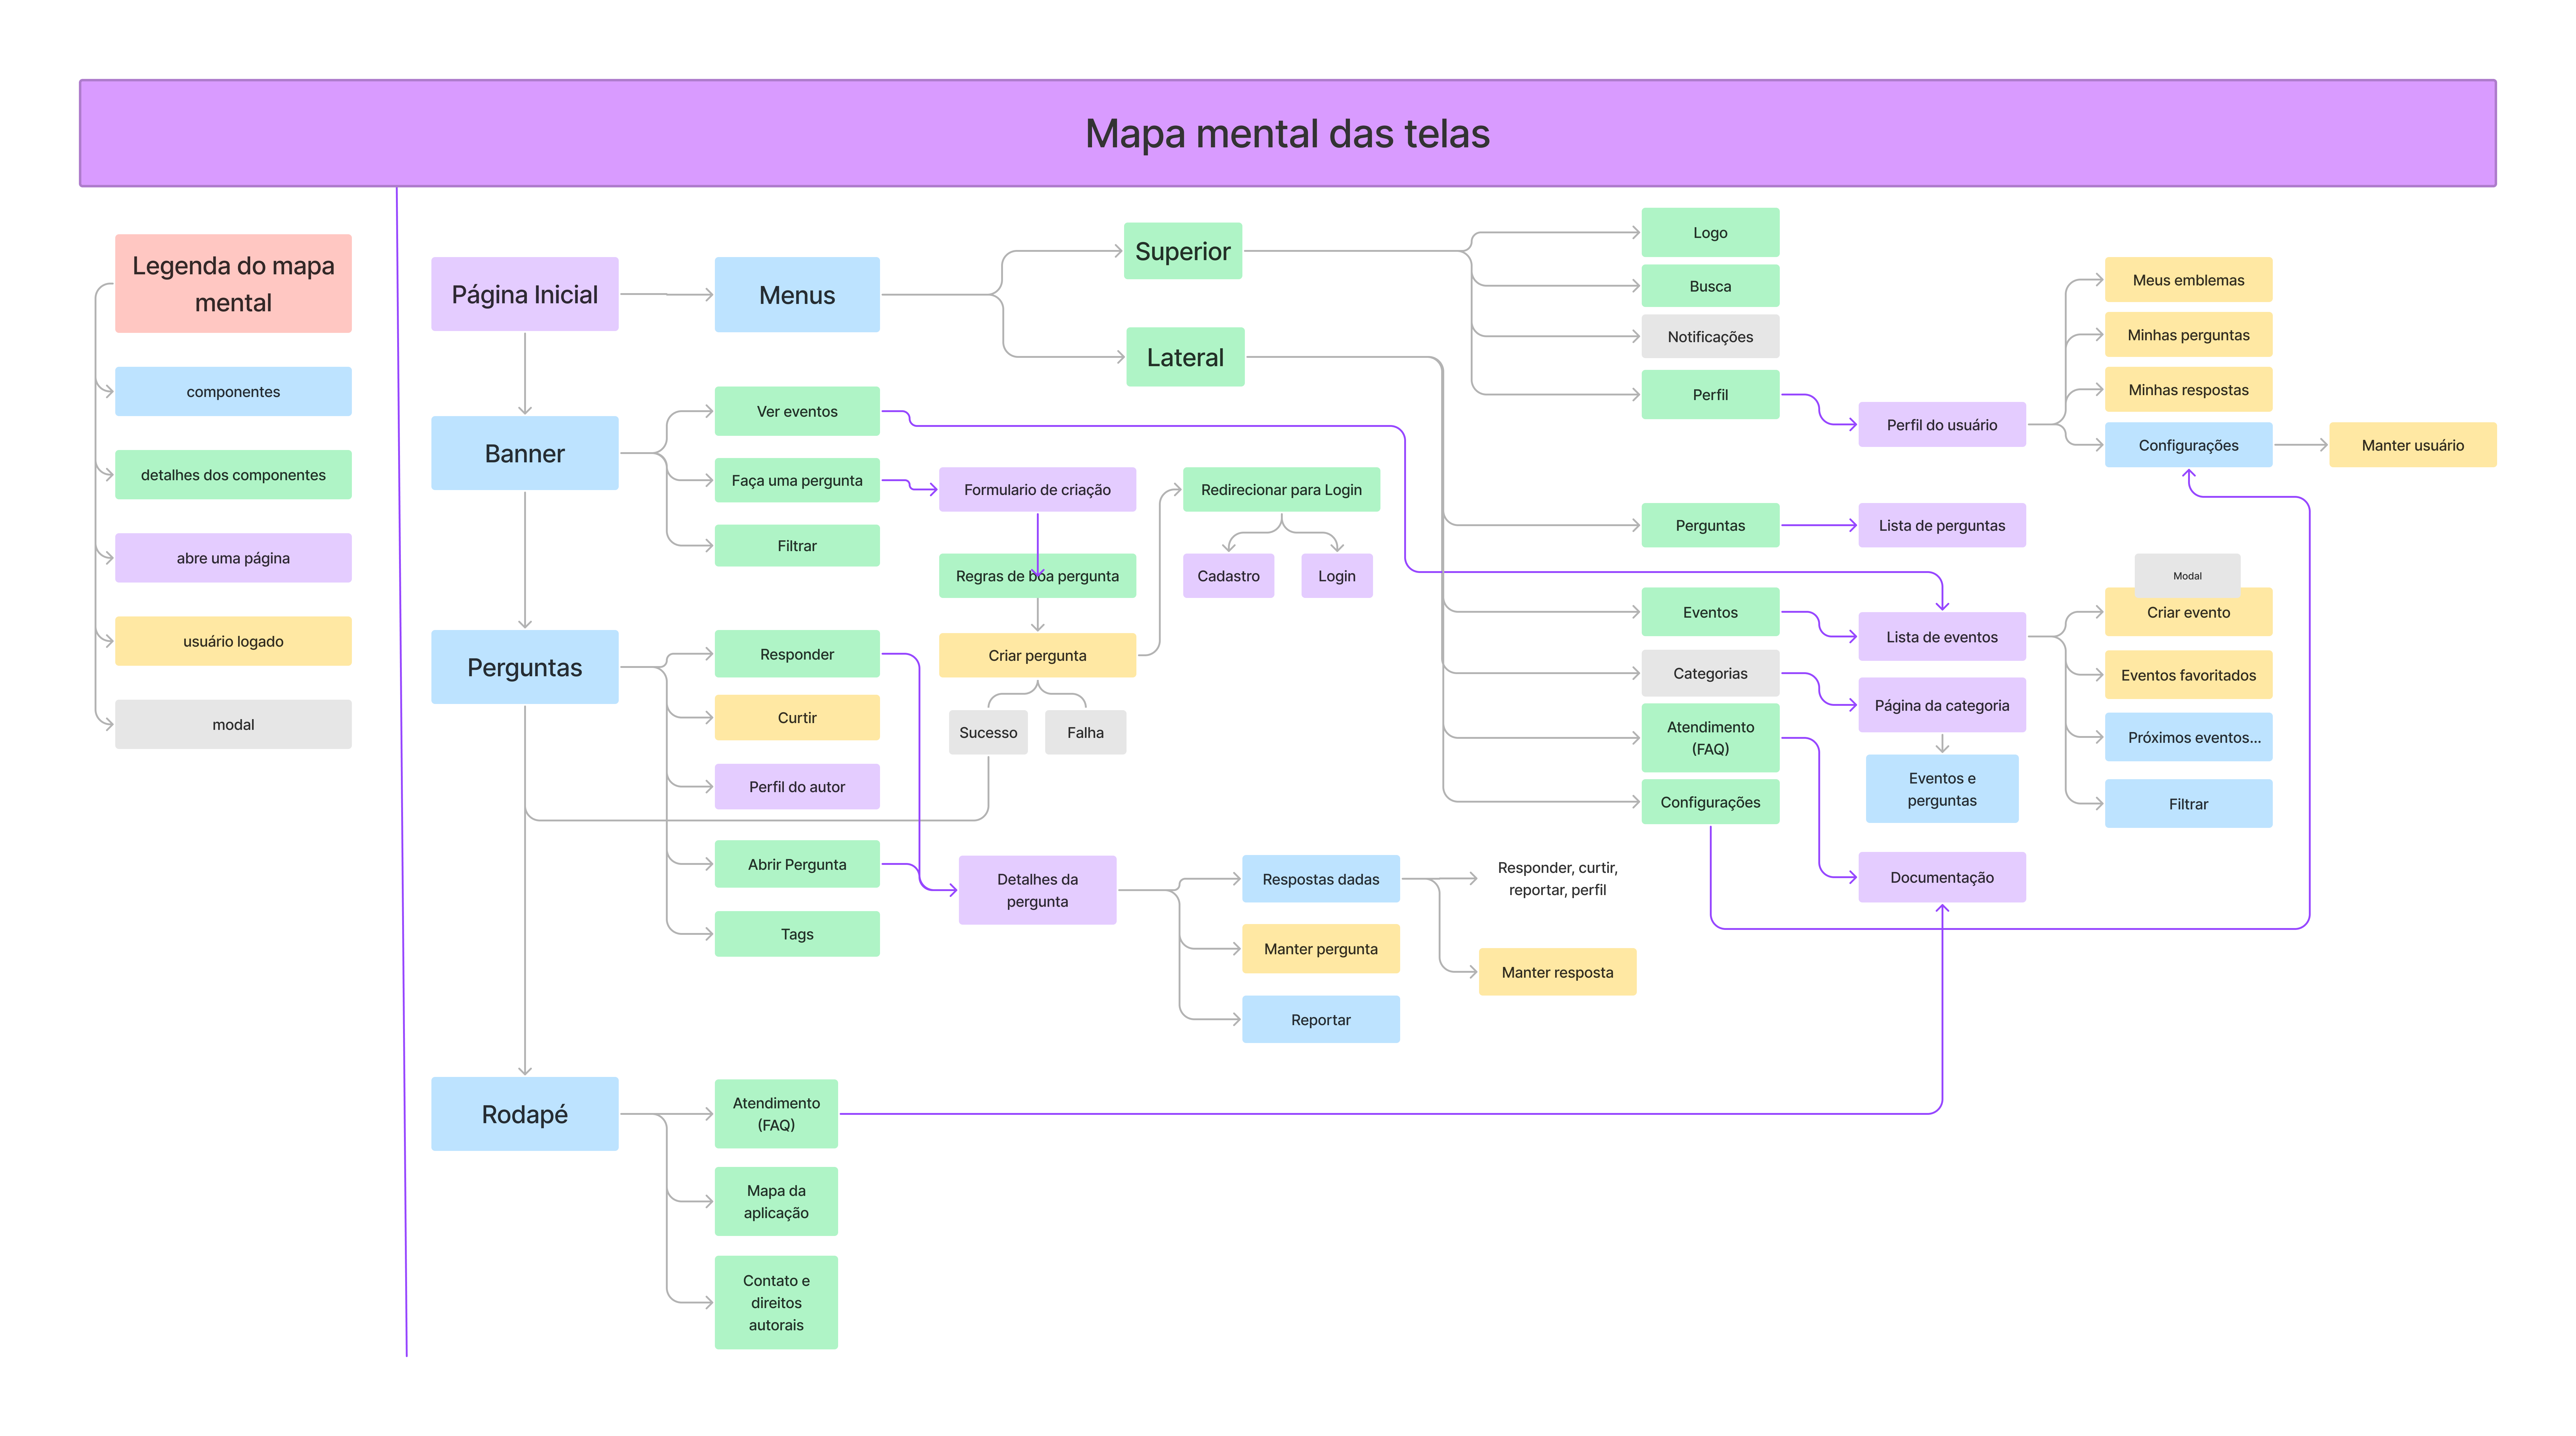
\includegraphics[width=1\textwidth]{anexos/Imagens_Prototipo/Mapa_Mental.png}
\fonte{os autores}
\end{figure}
\FloatBarrier

\subsection{Protótipos de alta fidelidade}
Nesta seção estão contidas as figuras que representam as principais telas do sistema em relação a \gls{POC} do projeto, cada tela apresenta uma breve contextualização sobre o seu conteúdo. De todo modo, a apresentação pode ser visualizada também pelo \href{https://www.figma.com/proto/GhIlybDubGmr3NkRU0a9GP/Protótipo---IFriends?node-id=73\%3A321}{Figma}.

A \autoref{Home Page} apresenta a página inicial do projeto, onde o usuário entra em contato pela primeira vez com o sistema. Nela o usuário pode navegar através de dois menus disponíveis na página: o lateral e o superior, usar a barra de pesquisa, \textit{logar} no seu perfil, acessar as suas configurações, entre outras ações disponibilizadas. Na página encontram as questões mais relevantes da comunidade, assim como os espaços destinados para a realização de uma pergunta ou de uma monitoria.

\begin{figure}[htb]
\centering
\caption{\label{Home Page} Página inicial}
\includesvg[inkscapelatex=false,width=0.7\textwidth]{anexos/Imagens_Prototipo/Home_Page.svg}
\fonte{os autores}
\end{figure}
\FloatBarrier

Quando o usuário clica em uma pergunta ou em ``Responder'' ele é direcionado à página dessa pergunta como mostra a \autoref{Pergunta e respostas}, nela ele pode encontrar as respostas já fornecidas por outros membros da comunidade, assim como também pode deixar a sua contribuição.

\begin{figure}[htb]
\centering
\caption{\label{Pergunta e respostas} Pergunta e respostas}
\includesvg[inkscapelatex=false,width=0.9\textwidth]{anexos/Imagens_Prototipo/Pergunta_Respostas.svg}
\fonte{os autores}
\end{figure}
\FloatBarrier

Já a \autoref{Cadastro de perguntas} corresponde a página de cadastro de perguntas, nessa tela são apresentados todos os elementos julgados necessários para a sua realização, nesta página ainda de encontra o manual de uma boa pergunta, tal foi elaborado com o intuito de ajudar e auxiliar o usuário na preparação de sua problemática. 

\begin{figure}[htb]
\centering
\caption{\label{Cadastro de perguntas} Cadastro de perguntas}
\includesvg[inkscapelatex=false,width=0.9\textwidth]{anexos/Imagens_Prototipo/Cadastro_Perguntas.svg}
\fonte{os autores}
\end{figure}
\FloatBarrier

As telas apresentadas até o momento são aquelas que se encontram relacionadas com a \gls{POC}, portanto vale salientar que esta seção será atualizada futuramente conforme o andamento e elaboração do projeto.


%---------------------------------------------------------------------------------------





